\documentclass[12pt, aspectratio=169]{beamer} % aspectratio = either 43 or 169
\usepackage[utf8]{inputenc}
\usepackage{graphicx}
\usepackage[T1]{fontenc}
\graphicspath{ {./img/} }

\usetheme{Hannover}
\mode<presentation>

% title and author
\title{A study of the use of complexity measures in the similarity search process adopted by kNN algorithm for time series prediction}
\author{Parmezan y Batista. 14th International Conference on Machine Learning and Applications (ICMLA) 2015}
\date{2021-03-16}
% document
\begin{document}


\frame{\titlepage}


\begin{frame}{Overview}
\tableofcontents
\end{frame}

\section{Introducción}

\begin{frame}{El problema de la predicción}
  \begin{itemize}
  \item La predicción del futuro siempre ha sido un problema.
  \item Toda serie temporal contiene un conjunto de patrones ocultos e interacciones difíciles de identificar e interpretar.
  \item Los algoritmos actuales:
    \begin{enumerate}
    \item Asumen e identifican características de los datos de la serie temporal.
    \item Generan un modelo explicativo para los datos actuales.
    \item Mediante extrapolación permiten hacer predicciones.
    \end{enumerate}
  \item Existen dos grandes filosofías de aproximación: \textbf{paramétricas} y \textbf{no paramétricas}
  \end{itemize}
\end{frame}

\begin{frame}{Tipos de aproximaciones al problema}
  \begin{block}{Aproximaciones paramétricas}
    Basados principalmente en modelos de autorregresión y medias móviles
    \[ y'_t = c + \varphi_1y'_{t-1} + \ldots + \varphi_py'_{t-p} +
          \theta_1\varepsilon_{t-1} + \ldots + \theta_q\varepsilon_{t-q} + \varepsilon_t\]
  \end{block}

  \begin{block}{Aproximaciones no paramétricas / Machine Learning}
    \begin{itemize}
    \item Enfoque \textbf{global}:
      \begin{itemize}
      \item Se entrena el modelo utilizando toda la serie temporal.
      \item Ejemplos: Redes neuronales y Support Vector Machine.
      \end{itemize}
    \item Enfoque \textbf{local}:
      \begin{itemize}
      \item Se buscan similitudes entre secciones de la serie temporal.
      \item Ejemplos: Técnicas Nearest Neighbours (kNN).
      \end{itemize}
    \end{itemize}

  \end{block}

\end{frame}

\section{kNN en series temporales}

\begin{frame}{kNN en series temporales}
  Esta aproximación busca similitudes en todo el histórico de la serie y realiza predicciones en base a la serie o series más similares.
  La predicción busca las \textit{k} (3) series más similares de \textit{l}(25) elementos. 
  \begin{figure}
  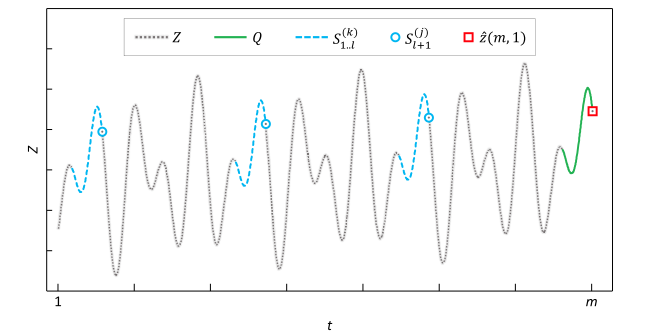
\includegraphics[width=8cm]{20210312_1_knn_summary.png}
  \label{fig:ejemplo_knn_ts}
\end{figure}

\end{frame}

\begin{frame}{Los tres grandes problemas de kNN}

  \begin{itemize}
  \item Problema 1: Amplitud y desfase.
  \item Problema 2: Gestión de la varianza en los objetos complejos.
  \item Problema 3: Tratamiento de las asociaciones triviales.
  \end{itemize}

  \begin{figure}
    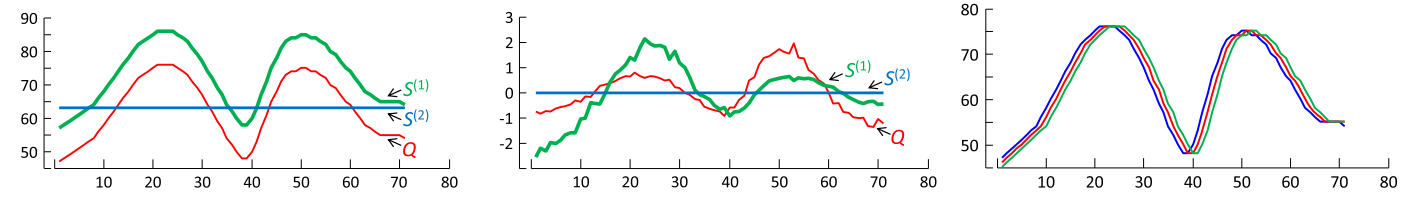
\includegraphics[width=1\textwidth]{20210313_1_tres_metricas.png}
  \end{figure}
  
\end{frame}

\begin{frame}{Los tres grandes problemas}{Problema 1: Amplitud y desfase}
  La secuencia S\textsuperscript{1} es igual a la secuencia a testear (Q) más un pequeño desfase.
  El error acumulado por la diferencia de amplitudes y desfases provoca penalizaciones importantes.

  \begin{figure}
      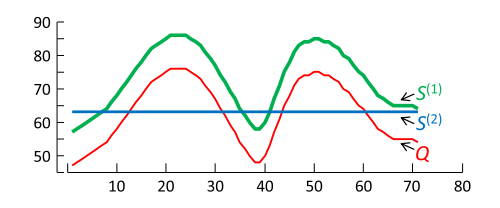
\includegraphics[width=8cm]{20210312_2_problema_offset.png}
      \label{fig:problema_1}
  \end{figure}
  En este caso se considera S\textsuperscript{2} más similar a Q que S\textsuperscript{1}.
\end{frame}

\begin{frame}{Los tres grandes problemas}{Problema 2:  Gestión de la varianza en los objetos complejos}
  La acumulación de errores menores debido a series con alta variabilidad intrínseca (objetos complejos) penaliza mucho contra los objetos simples.

  \begin{figure}
  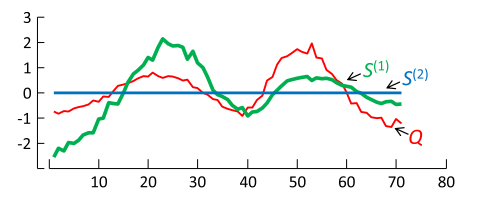
\includegraphics[width=8cm]{20210312_3_problema_complejos.png}
  \label{fig:problema_2}
\end{figure}

  En este caso la secuencia simple S\textsuperscript{2} se considera  más similar a Q que S\textsuperscript{1}.

\end{frame}

\begin{frame}{Los tres grandes problemas}{Problema 3: Tratamiento de las asociaciones triviales}
  En este caso las tres secuencias comparten muchas observaciones.
  Este caso ocurre cuando se incluye la secuencia a buscar en \textit{pool} de secuencias elegibles, o bien hay aciertos fortuitos.
  \begin{figure}
    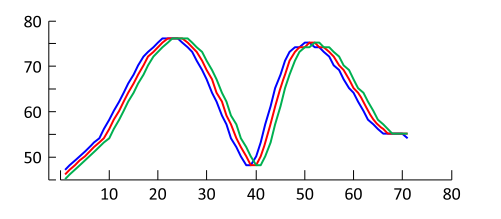
\includegraphics[width=8cm]{20210312_4_problema_triviales.png}
    \label{fig:problema_3}
  \end{figure}
  
\end{frame}

\begin{frame}{Los tres grandes problemas}{Soluciones}
  \begin{block}{Problema 1: Amplitud y desfase}
    Solución: Transformar las series para que sean invariantes en amplitud y desfase. Por ejemplo aplicando la \textit{z-normalización}.
    \[  z'_t = \frac{z_t - \mu}{\sigma} \]
  \end{block}
  \begin{block}{Problema 2: Gestión de la varianza en los objetos complejos}
    Solución: Usar una distancia invariante a la complejidad (CID). 
  \end{block}

  \begin{block}{Problema 3: Tratamiento de las asociaciones triviales}
    Solución: Excluir automáticamente las asociaciones triviales, en este caso utilizando un chequeo iterativo y evitando solapamientos.
  \end{block}
\end{frame}

\begin{frame}{kNN-TSPI}{Una propuesta de adaptación de kNN en el problema de la predicción de las series temporales}
  \begin{columns}
    \begin{column}{0.5\textwidth}
      El algoritmo kNN-Time Series Prediction with Invariances (kNN-TSPI) es una variante del kNN que tiene en cuenta las soluciones de los tres problemas anteriores:

      \begin{itemize}
      \item Problema 1: Z-normalización en la línea 3
      \item Problema 2: Aplicación de la distancia invariante en la línea 5*
      \item Problema 3: Identificación de los \textit{k} vecinos más cercanos en la línea 6
      \end{itemize}
      
    \end{column}
    \begin{column}{0.5\textwidth}
        \begin{figure}
          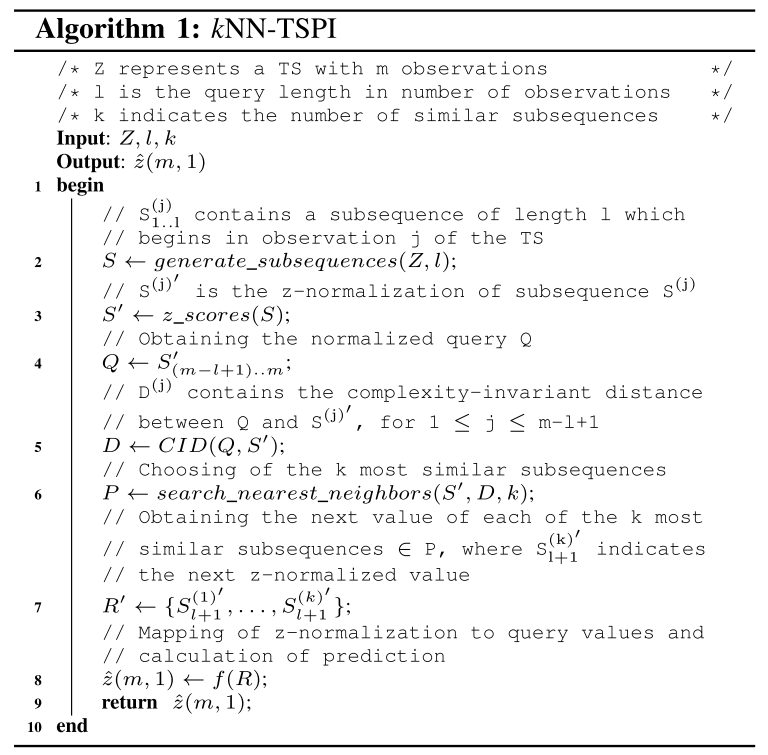
\includegraphics[width=0.8\textwidth]{20210313_2_algoritmo.png}
          \label{fig:algoritmo}
        \end{figure}
    \end{column}                
  \end{columns}
  Este es un algoritmo de complejidad $O(m\cdot l)$
  
\end{frame}


\section{Estudio de las métricas de complejidad}

\begin{frame}{Notas sobre la CID}{Definición de la CID}
  La distancia de complejidad invariante usa iformación sobre la distancia euclideana (ED) ajustada por un factor de complejidad (CF).
  Este factor de complejidad se calcula, en este caso, a partir de una estimación de la complejidad cuadrática (CE). 

  \[ CID(Q,C) = ED(Q,C) \times CF(Q,C) \]

  \[ CF(Q,C) = \frac
    { \max{ (CE(Q),CE(C))} }
    { \min{(CE(Q),CE(C))}  }
  \]

  \[ CE(Q) = \sqrt{ \sum_{i=1}^{n=1}{  ( q_i - q_{i+1} )^2 } }  \]

\end{frame}

\begin{frame}{Notas sobre la CID}{¿Qué métrica utilizar}
  \begin{itemize}
  \item \textbf{Diferencia cuadrática.}
  \item \textbf{Diferencia absoluta.}
  \item \textbf{Compresión}: Aproximación de la complejidad de Kolmogorov usando el algoritmo de compresión LempelZiv.
  \item \textbf{Vértices (Edges)}: Número de vértices en los segmentos, se interpreta como cambios de tendencia.
  \item \textbf{Zero-crossing}: Número de veces que la señal cambia de signo.
  \item \textbf{Permutation-Entropy}: Combinación de patrones en la señal.
  \end{itemize}
\end{frame}

\begin{frame}{Notas sobre la CID}{Evaluación empírica}
  Se evalúan las seis medidas presentadas junto con la distancia euclideana no ajustada.
  \begin{columns}
    \begin{column}{0.5\textwidth}
      \begin{itemize}
        \item Paso 1: Selección de 55 series del repositorio ICMC-USP TSPR.
        \item Paso 2: Se estiman los parámetros usando el método de Mean Square Error y se realizan las predicciones.
        \item Paso 3: Se comparan usando: MAPE, Coeficiente Theil U y POCID.
      \end{itemize}
    \end{column}

    \begin{column}{0.5\textwidth}
      \begin{figure}
        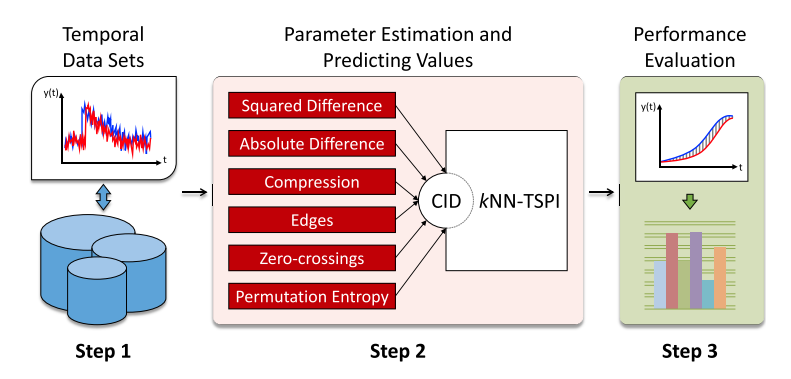
\includegraphics[width=\textwidth]{20210313_3_evaluacion_cid.png}
      \end{figure}
    \end{column}

    \end{columns}
  
\end{frame}


\begin{frame}{Evaluación empírica de las distancias}{MAPE}
  \begin{figure}
    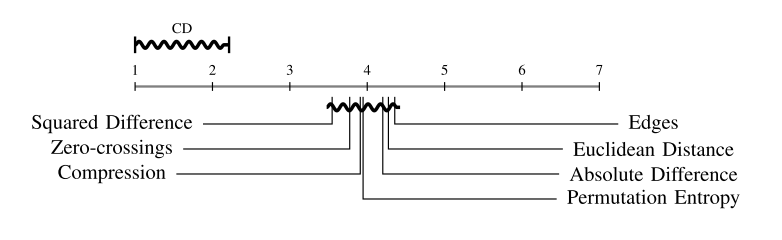
\includegraphics[width=0.6\textwidth]{20210313_4_nemenyi_distancias_cd.png}
  \end{figure}
\end{frame}

\begin{frame}{Evaluación empírica de las distancias}{POCID y Theil U}
  \begin{figure}
    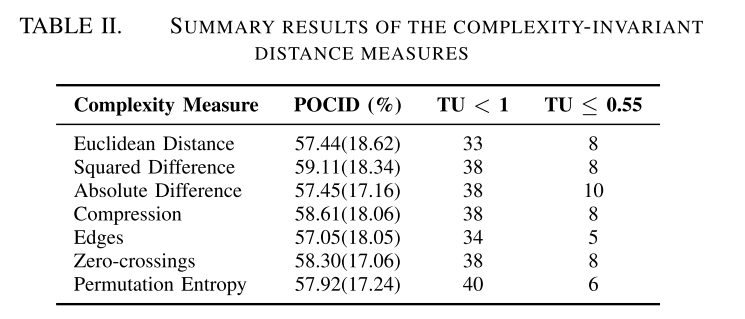
\includegraphics[width=0.6\textwidth]{20210313_5_tabla_cid.png}
  \end{figure}
\end{frame}


\section{Comparación de kNN-TSPI con otras técnicas no paramétricas}

\begin{frame}{Comparando kNN-TSPI con SVM y MLP}{Hipótesis y diseño experimental}

  \begin{block}{Hipótesis a contrastar}
    ¿Existen diferencias significativas entre kNN-TSPI y los métodos de Machine Learning más utilizados?
  \end{block}

  \begin{block}{Diseño experimental}
    \begin{itemize}
    \item \textbf{Modelos comparados}: Multilayer Perceptron (ML) y Support Vector Machine (SVM)
    \item \textbf{Tunning} 10-fold cross validation
    \item \textbf{Métricas de validación}: MAPE, POCID y Theil U.
    \end{itemize}
  \end{block}
  
\end{frame}

\begin{frame}{Comparando kNN-TSPI con SVM y MLP}{Resultados}
  \begin{figure}
    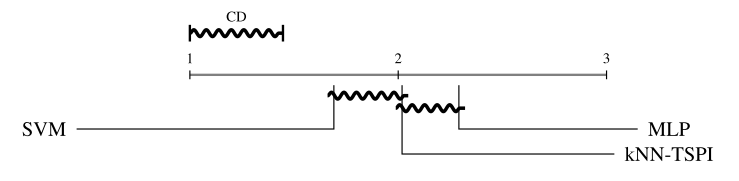
\includegraphics[width=\textwidth]{20210314_1_nemnyi_distancias_tecnicas_cd.png}
  \end{figure}
\end{frame}


\section{Conclusiones}

\begin{frame}{Discusión}
  \begin{block}{Resumen del trabajo realizado}

    \begin{itemize}
    \item Se presenta un nuevo método de predicción de series temporales basado en similaridad y que corrige los problemas del desfase/amplitud; complejidad invariantes y tratammiento de los aciertos triviales.
    \item Se analizan 6 aproximaciones para tratar el problema de la complejidad invariante, identificando como buena opción la diferencia cuadrática.
    \item Se compara el método con SVM y MLP. No muestra diferencias significativas con SVM y mejora MLP.
    \end{itemize}
  \end{block}

  \begin{block}{Trabajo futuro}
    \begin{itemize}
    \item Continuar analizando las propiedades de kNN-TSPI.
    \item Comparar el algoritmo contra los métodos más utilizados, como el ARIMA.
    \end{itemize}

  \end{block}

\end{frame}


\begin{frame}{}
  \centering \Large
  \emph{Muchas gracias, ¿preguntas?}
\end{frame}

\end{document}